\section {Grundlagen}
In diesem Abschnitt wird zunächst der Greifarm OpenMANIPULATOR-X vorgestellt.
Anschließend wird eine Übersicht über die wichtigsten Komponenten des Betriebssystems gegeben, mit dem dieser Greifarm läuft.
Weiterhin werden die theoretischen Grundlagen der Planung dargestellt, die zur Steuerung des Greifarms genutzt werden sollen.
Abschließend wird das System erklärt, das Planung und Roboter kombiniert.
\subsection{OpenMANIPULATOR-X}
Der OpenMANIPULATOR-X ist ein von der Firma ROBOTIS{\footnote{http://en.robotis.com}} nach den Prinzipien ``OpenSoftware`` und ``OpenHardware`` hergestellter Greifarm.
OpenSoftware steht hierbei dafür, dass es ein OpenSource Projekt ist und auf dem OpenSource Projekt \ac{ROS2} basiert.
OpenHardware steht dafür, dass die meisten Komponenten als STL-Dateien zur Verfügung stehen und als Ersatzteile oder zum Anpassen des Greifarms mittels eines 3D-Druckers selbst hergestellt werden können.\\
Der OpenMANIPULATOR-X ist eine 5DOF (5 Degrees of Freedom) Plattform, die mittels 5 Servomotoren{\footnote{Modelbezeichnung: DYNAMIXEL XM430-W350-T}} gesteuert wird.
Dies ist aufgeteilt in 4DOF für den Arm sowie 1DOF für den Greifer.
Es kann eine Last bis 500g getragen werden.
\subsection{ROS2}
\acf{ROS2} ist eine Sammlung von Bibliotheken und Werkzeugen für Robotik-Applikationen, die alle OpenSource sind.
Die erste \ac{ROS2} Release-Version erschien im Dezember 2017 unter dem Namen ''Ardent Apalon''.\\
Es werden  mehrere \acp{RCL}  zur Verfügung gestellt, die den Zugriff auf die \ac{ROS2}-API ermöglichen.
Die \acp{RCL} für die Sprachen C++ und Python (rclcpp und rclpy) werden dabei direkt vom \ac{ROS2}-Team verwaltet.
Von der Community wurden weitere \acp{RCL}, unter anderem für die Sprachen C\#, Swift und Rust, entwickelt.\\
Um die Entwicklung der \acp{RCL} zu vereinfachen und die Logik sprachunabhängig zu machen werden Funktionalitäten als C Interfaces zugänglich gemacht, für die in den \acp{RCL} Wrapper geschrieben werden.\\
Die grundlegende Komponente einer \ac{ROS2} Anwendung ist die Node.
Typischerweise besteht eine Anwendung aus mehreren Nodes.
Entsprechend dem Prinzip \emph{Separation of Concerns} (Trennung der Zuständigkeiten) sollen Nodes so implementiert werden, dass sie jeweils nur eine spezifische Aufgabe haben.
\subsubsection{Interfaces}
In diesem Abschnitt werden die verschiedenen Arten von Interfaces beschrieben, die für die im folgenden Abschnitt~\ref{rosnodecomm} erklärten Methoden zur Kommunikation zwischen mehreren Nodes genutzt werden.\\
\ac{ROS2}-Interfaces definieren, welche Daten gesendet werden und welchen Datentyp diese haben.
Sie werden in der \ac{IDL} geschrieben, die es ermöglicht automatisch Quellcode in verschiedenen Sprachen für diese zu generieren.\\

\textbf{Message} Eine Message ist die einfachste Art der \ac{ROS2}-Interfaces, die gleichzeitig auch ein Baustein für die anderen Interfaces sein wird.\\
Message-Definitionen haben die Dateiendung \verb|.msg| und werden per Konvention in einem Ordner \verb|msg/| gespeichert.
Jede \verb|.msg| Datei besteht aus den folgenden Teilen:
\begin{itemize}
\item Felder
\item Konstanten
\end{itemize}
Konstanten sind optional und es gibt mindestens ein Feld.
Jedes Feld besteht aus einem Datentyp und einem durch ein Leerzeichen getrennten Namen: \verb|typ name|, z.B. \verb|bool isDone|.
Als Datentyp können dabei die integrierten Datentypen (s. Tabelle~\ref{tab:builtintypes}) oder der Name anderer Messages genutzt werden.
Zusätzlich kann jeder integrierte Datentyp als Array definiert werden (s. Tabelle~\ref{tab:arraytypes}).\\
Feldnamen müssen kleingeschrieben sein.
Es können alphanumerische Zeichen sowie der Unterstrich zur Trennung von Wörtern genutzt werden.
Das erste Zeichen muss ein Buchstabe sein und der Name darf nicht mit einem Unterstrich enden.
Zusätzlich darf es keine aufeinander folgende Unterstriche geben.\\
Konstanten behalten das Format der Felder bei.
Der Name der Konstante wird komplett in Großbuchstaben geschrieben.
Zusätzlich bekommen Konstanten einen Wert zugewiesen, der nicht innerhalb des Programms geändert werden kann.
Die Zuweisung des Wertes erfolgt mit dem ''\verb|=|'' Zeichen: \verb|string EXAMPLE="test"|.
\begin{table}[ht]
    \centering
    \caption{Integrierte Datentypen für Interfaces und deren C++ Equivalent}
\begin{tabular}{|l|l|}
\hline
\textbf{Typ} & \textbf{C++}   \\ \hline
bool         & bool           \\ \hline
byte         & uint8\_t       \\ \hline
char         & char           \\ \hline
float32      & float          \\ \hline
float64      & double         \\ \hline
int8         & int8\_t        \\ \hline
uint8        & uint8\_t       \\ \hline
int16        & int16\_t       \\ \hline
uint16       & uint16\_t      \\ \hline
int32        & int32\_t       \\ \hline
uint32       & uint32\_t      \\ \hline
int64        & int64\_t       \\ \hline
uint64       & uint64\_t      \\ \hline
string       & std::string    \\ \hline
wstring      & std::u16string \\ \hline
\end{tabular}
    \label{tab:builtintypes}
\end{table}
\begin{table}[ht]
    \centering
    \caption{Array Typen und deren C++ Equivalent}
\begin{tabular}{|l|l|}
\hline
\textbf{Typ} & \textbf{C++}   \\ \hline
static array               & std::array<T, N>   \\ \hline
unbounded dynamic array    & std::vector        \\ \hline
bounded dynamic array      & custom\_class<T, N> \\ \hline
bounded string             & std::string        \\ \hline
\end{tabular}
    \label{tab:arraytypes}
\end{table}

\textbf{Service} Service-Definitionen beschreiben eine Anfrage und eine Antwort.
Die Definition hat die Dateiendung \verb|.srv| und wird im Ordner \verb|srv/| gespeichert.
Anfrage und Antwort werden innerhalb der Datei durch ''\verb|---|'' getrennt.
Für beide Teile gilt, dass sie gültig sind, wenn sie einer gültigen Message-Definition entsprechen.
Ein Beispiel einer einfachen Service-Definition ist in Listing~\ref{lst:serviceexample} gegeben.\\
\begin{minipage}{\linewidth}%minipage to prevent page break
\begin{lstlisting}[caption={Beispiel einer Service-Definition}, label={lst:serviceexample}]
int32 request_int_name
string request_string_name
---
float32 response_float_name
\end{lstlisting}
\end{minipage}

\textbf{Action} Action-Definitionen bestehen aus den 3 Teilen Anfrage, Antwort und Feedback, in dieser Reihenfolge.
Wie auch für Service-Definitionen gilt, dass die Teile durch ''\verb|---|'' getrennt sind und jeder einzelne Teil gültig ist, wenn er einer gültigen Message-Definition entspricht.

\subsubsection{Node-Kommunikation}{\label{rosnodecomm}}
Damit verschiedene Nodes untereinander kommunizieren können, gibt es verschiedene Methoden, die sich darin unterscheiden, in welche Richtungen Nachrichten gesendet werden und ob es eine direkte Reaktion gibt.
Für alle Methoden gilt, dass sie von einer Node unter einem bestimmten Namen sowie einem Typ zur Verfügung gestellt werden und von anderen Nodes durch eben diese genutzt werden können.\\

\textbf{Topic} Topics entsprechen in etwa einem Newsletter System: eine Node veröffentlicht Daten (Publisher), die von allen anderen Nodes (Subscriber) empfangen werden, die sich für diese registriert haben (s. Abbildung~\ref{fig:topic}).
Das Format der Daten entspricht einer gewählten Message-Definition.\\

\begin{figure}[ht!]
    \centering
    \begin{tikzpicture}[node distance=5cm,every node/.style={circle, draw, minimum size=1.5cm}]

    \node (1) at (0,0) [text width=2cm,align=center,circle,draw] {Publisher};
    \node (2) at (10,0) [text width=2cm,align=center,circle,draw,right of=1] {Subscriber};

    \path[-{Latex[length=3mm]},every node/.style={font=\sffamily\small}]
    (1) edge[bend left] node [midway,above] {Nachricht (Message)} (2)
    \end{tikzpicture}
    \caption{Nachrichtenfluss eines Topic}
    \label{fig:topic}
\end{figure}
\textbf{Service und Client} Services werden für Prozesse genutzt, in denen eine Anfrage gesendet und eine Antwort erwartet wird.
Ein Client sendet die Anfrage an den Service, der eine Antwort zurückgibt (s. Abbildung~\ref{fig:service}).
Als Typ wird eine Servicedefinition genutzt.\\

\begin{figure}[ht!]
    \centering
    \begin{tikzpicture}[node distance=5cm,every node/.style={circle, draw, minimum size=2cm}]

        \node (1) at (0,0) [text width=2cm,align=center,circle,draw] {Client};
        \node (2) at (10,0) [text width=2cm,align=center,circle,draw,right of=1] {Service};

        \path[-{Latex[length=3mm]},every node/.style={font=\sffamily\small}]
        (1) edge[bend left] node [midway,above] {Anfrage (Request)} (2)
        (2) edge[bend left] node [midway,below] {Antwort (Response)} (1)
    \end{tikzpicture}
    \caption{Nachrichtenfluss eines Service}
    \label{fig:service}
\end{figure}
\textbf{Action Server und Client} Actions sind für länger andauernde Prozesse gedacht.
Eine Node erstellt einen Action Server über den eine Action zur Verfügung gestellt wird.
Andere Nodes können über einen Action Client eine Anfrage senden.
Der Server bearbeitet die Anfrage und sendet bei Beendigung eine Antwort mit einem Ergebnis an den Client.
Während der Dauer der Action kann der Server den Client optional mit Feedback-Nachrichten über den aktuellen Status informieren.
Dieser Nachrichtenfluss wird in Abbildung~\ref{fig:action} gezeigt.\\
Als Typ wird eine Action Definition genutzt.\\
\begin{figure}[ht!]
    \centering
    \begin{tikzpicture}[node distance=5cm,every node/.style={circle, draw, minimum size=2cm}]

        \node (1) at (0,0) [text width=2cm,align=center,circle,draw] {Action Client};
        \node (2) at (10,0) [text width=2cm,align=center,circle,draw,right of=1] {Action Server};

        \path[-{Latex[length=3mm]},every node/.style={font=\sffamily\small}]
        (1) edge[bend left] node [midway,above] {Anfrage (Request)} (2)
        (2) edge[bend left] node [midway,below] {Antwort (Response)} (1)
        (2) edge[bend left=10] node [midway,below] {Feedback} (1)
    \end{tikzpicture}
    \caption{Nachrichtenfluss einer Action}
    \label{fig:action}
\end{figure}
\subsection {Planung}
Planung (auch Handlungsplanung) ist ein Bereich der Künstlichen Intelligenz, der sich mit der Lösung von Planungs- und Schedulingproblemen befasst~\cite{aiplanning}.
\subsubsection{Stanford Research Institute Problem Solver}{\label{chap:strips}}
Der \emph{\ac{STRIPS}} ist ein automatischer Planer, der von Richard Fikes und Nils Nilsson 1971 entwickelt wurde~\cite{FIKES1971189}.
Mit dem gleichen Namen wird auch die Sprache bezeichnet, die als Eingabe für diesen Planer genutzt wird.
In diesem Abschnitt wird zunächst auf die Sprache eingegangen, die die Grundlage vieler weiterer Sprachen zur Darstellung von Planungsdomänen und -problemen ist.
Anschließend wird der von \ac{STRIPS} genutzte Algorithmus beschrieben.\\
Ein \ac{STRIPS}-Modell besteht aus 3 Teilen:
\begin{itemize}
    \item Startzustand
    \item Ziele
    \item Aktionen
\end{itemize}
Aktionen bestehen wiederum aus:
\begin{itemize}
    \item Vorbedingungen
    \item Effekten
\end{itemize}
Ein \ac{STRIPS}-Modell kann mathematisch als 4-Tupel \((P,O,I,G)\) beschrieben werden \cite{stripsdef}:
\begin{enumerate}
    \item \(P\): eine endliche Menge von Bedingungen
    \item \(O\): eine endliche Menge von Aktionen (auch Operatoren) mit der Form $Pre \Rightarrow Post$:
    \item \(I\): der Startzustand, $I\subseteq P$
    \item \(G\): eine endliche Menge von Zielen
\end{enumerate}
Es gilt die \emph{Closed World Assumption (CWA)}: alles was nicht explizit als wahr beschrieben ist, gilt als falsch.\\
$P$ ist die Menge aller Bedingungen, die relevant sind.
Jeder Zustand ist eine Teilmenge $S\subseteq P$.\\
$O$ ist die Menge der Aktionen die einen Zustand in einen anderen ändern können.
Aktionen sind 4-Tupel \((o^+,o^-,o_+,o_-)\), bei dem jedes Element eine Menge von Bedingungen sind.
Die ersten zwei Mengen beschreiben die Vorbedingungen ($Pre$): Bedingungen, die wahr sein müssen ($o^+$) sowie Bedingungen, die falsch sein müssen ($o^-$).
Die letzten beiden Mengen beschreiben den Effekt, den die Aktion nach ihrer Ausführung auf einen Zustand hat ($Post$): Bedingungen, die wahr werden ($o_+$) und Bedingungen, die falsch werden ($o_-$).\\
$I$ beschreibt, welche Bedingungen anfangs wahr oder falsch sind.
Eine Bedingung $p\in P$ ist anfangs wahr, wenn $p\in I$ und sonst falsch.\\
$G$ ist die Menge der Bedingungen, die erreicht werden soll, bestehend aus den Zielen, die wahr sein sollen ($G_+$) und denen, die falsch sein sollen ($G_-$).
Ein Zustand $S\subseteq P$  ist ein Zielzustand, wenn $G_+\subseteq S$ und $G_-\cap S =\emptyset$.\\
Ein Plan besteht aus einer Menge von Aktionen, die vom Startzustand zu einem Zielzustand führen.
Dieser Plan ist ein \emph{Total-Order} Plan: alle Aktionen haben eine feste Reihenfolge innerhalb des Plans.
Um einen Plan zu finden, wird ein Suchbaum erstellt.
Die Suche findet im Zustandsraum statt.
Jeder Knoten ist ein Zustand.
Jede Kante ist die Aktion, um den Zustand bzw. Knoten, von der die Kante ausgeht, zu dem Zustand zu überführen, zu dem die Kante geht.
Es wird die GPS Strategie angewandt, um Unterschiede zwischen dem aktuellen Zustand und dem Ziel zu extrahieren und relevante Aktionen für diese Unterschiede zu finden~\cite{FIKES1971189}.\\
\ac{STRIPS} beginnt damit, das Ziel $G_0$ für den Startzustand $M_0$ zu beweisen.
Gelingt dies, ist das Ziel bereits erreicht und kein Plan notwendig.
Ist das Ziel nicht beweisbar, wird der Unterschied zwischen $M_0$ und $G_0$ ermittelt und von diesem aus weiter gesucht.
Es wird eine Aktion gesucht, die diesen Unterschied weiter verringern kann.
Vorbedingungen dieser Aktion werden als Unterziel genutzt.
Kann ein (Unter)Ziel für den Zustand $M_0$ bewiesen werden, werden die Effekte der Aktion auf $M_0$ angewandt und es entsteht ein Zustand $M_1$.
Dieses Verfahren wiederholt sich bis ein Zustand entsteht, in dem das Ziel $G_0$ bewiesen werden kann.
\subsubsection{Planning Domain Definition Language}
Die \emph{\ac{PDDL}} ist eine Sprache zur Modellierung von Planungsaufgaben.
Im Rahmen dieser Arbeit wird nicht auf alle Aspekte von \ac{PDDL} eingegangen.
Der Fokus liegt auf einigen grundlegenden Teilen sowie auf den genutzten Erweiterungen.\\
Die Beschreibung des Problems setzt sich aus folgenden grundlegenden Komponenten zusammen:
\begin{itemize}
    \item Objekt
    \item Prädikat
    \item Startzustand
    \item Aktion
    \item Ziel
\end{itemize}
Objekte sind Dinge in der Welt, die für die Planung relevant sind.
Dies können bspw.\ Orte oder Personen sein und werden in \ac{PDDL} entsprechend Listing~\ref{lst:pddlobjects} beschrieben.
\begin{lstlisting}[caption={Objektbeschreibung in \acs{PDDL}},language=pddl,label={lst:pddlobjects}]
(:objects kitchen supermarket
          fabian)
\end{lstlisting}
Prädikate sind Eigenschaften, die Objekte haben können.
Eine Person kann sich an einem Ort befinden oder eine bestimmte Größe haben (s. Listing~\ref{lst:pddlpredicates}).
\begin{lstlisting}[caption={Prädikatbeschreibung in \acs{PDDL}},language=pddl,label={lst:pddlpredicates}]
(:predicates (person_at ?person ?location)
            (tall ?person))
\end{lstlisting}
Der Startzustand ist die Beschreibung der Welt zu Beginn der Planungsaufgabe.
Er besteht aus einer Menge von Instanzen von Prädikaten, also Prädikate, die an Objekte gebunden sind (s. Listing~\ref{lst:pddlinit}).
\begin{lstlisting}[caption={Startzustand in \acs{PDDL}},language=pddl,label={lst:pddlinit}]
(:init (person_at fabian kitchen))
\end{lstlisting}
Aktionen sind die vorhandenen Möglichkeiten, den Zustand der Welt zu verändern.
Diese entsprechen den in Abschnitt~\ref{chap:strips} beschriebenen Aktionen mit einer Menge von Vorbedingungen und einer Menge von Effekten (s. Listing \ref{lst:pddlaction}).
\begin{lstlisting}[caption={Aktion, um eine Person von einem Ort zum anderen zu bewegen in \acs{PDDL}},language=pddl,label={lst:pddlaction}]
(:action move
    :parameters (?p ?loc_from ?loc_to)
    :precondition (and (person_at ?p ?loc_from))
    :effect (and (person_at ?p ?loc_to)
                (not (person_at ?p ?loc_from))))
\end{lstlisting}
Ein Ziel ist eine Menge von Instanzen, die am Ende der Planung Teil des Zustands der Welt sein soll (s. Listing~\ref{code:pddlgoal}).
\begin{lstlisting}[caption={Ziel in \acs{PDDL}},language=pddl,label=code:pddlgoal]
(:goal (and (person_at fabian supermarket))
\end{lstlisting}
Diese Komponenten werden aufgeteilt:
\begin{itemize}
    \item Domäne
    \item Problem
\end{itemize}
Die Domäne enthält die allgemeinen Rahmenbedingungen für das Problem: Prädikate und Aktionen.
Die Datei beginnt mit \verb|(define (domain name_der_domäne)|.\\
Das Problem enthält die Informationen zu einem spezifischen Problem: Objekte, den Startzustand und das Ziel.
Die Datei beginnt mit\\\verb|(define (problem name_des_problems) (:domain name_der_domäne)|.\\
Um sicherzustellen, dass nur bestimmte Objekte für bestimmte Parameter in Frage kommen (es kann mit der \emph{move} Aktion nur eine Person bewegt werden und der Start und das Ziel sind Orte) wurden ursprünglich weitere Prädikate genutzt, um Objekte zu typisieren.
Für das aktuelle Beispiel wären das die Prädikate \emph{location(x)} und \emph{person(x)}.
Die Aktion \emph{move} wird dann um entsprechende Vorbedingungen erweitert (s. Listing~\ref{lst:pddlactiontypepredicates}).
\begin{lstlisting}[caption={Move Aktion mit Prädikaten zur Typisierung},language=pddl,label={lst:pddlactiontypepredicates}]
(:action move
    :parameters (?p ?loc_from ?loc_to)
    :precondition (and (person ?p)
                        (location ?loc_from)
                        (location ?loc_to)
                        (person_at ?p ?loc_from))
    :effect (and (person_at ?p ?loc_to)
                (not (person_at ?p ?loc_from))))
\end{lstlisting}
Um dies zu vereinfachen, wurde mit \acs{PDDL} 2.1 unter anderem direkte Typisierung eingeführt.
In der Domäne werden die möglichen Typen deklariert, Objekte werden mit einem Typ initialisert und Aktionen können Parameter auf einen Typ beschränken (s. Listing~\ref{lst:pddltypes})
\begin{lstlisting}[caption={Typ Unterstützung in \acs{PDDL} 2.1},language=pddl,label={lst:pddltypes}]
(:types person
        location)
(:objects kitchen supermarket - location
          fabian - person)
(:action move
    :parameters (?p - person ?loc_from - location ?loc_to - location)
    :precondition (and (person_at ?p ?loc_from))
    :effect (and (person_at ?p ?loc_to)
                (not (person_at ?p ?loc_from))))
\end{lstlisting}
Eine weitere Neuerung in \ac{PDDL}2.1 ist die \emph{durative action} zur Modellierung von Aktionen mit einer Dauer für das temporale Planen.\\
Es wird jeder Aktion eine Dauer zugeordnet (\verb|:duration (= ?duration 0.25)|), die auch für Metriken genutzt werden kann.
Zusätzlich bekommen Bedingungen und Effekte einen temporalen Zusatz: \verb|at start| und \verb|at end| können sowohl für Bedingungen als auch Effekte benutzt werden, um festzulegen zu welchem Zeitpunkt der Aktion diese Bedingung zutrifft oder der Effekt eintritt.
Für Bedingungen gibt es außerdem \verb|over all|, damit eine Bedingung über die komplette Dauer der Aktion zutreffen muss, damit sie gültig ist.\\
Da Bedingungen dadurch nicht mehr strikt vor Ausführung der Aktion gelten müssen, wird das Schlüsselwort \verb|:precondition| zu \verb|:condition| geändert.

\subsubsection{\acs{PDDL}-Plugin für VS Code}
Im Marketplace von Visual Studio Code ist ein PDDL-Plugin von Jan Dolejsi verfügbar.
Dieses vereinfacht die Entwicklung und das Testen von Domänen und Problemen im \ac{PDDL}-Format.
Es beinhaltet Syntax-Highlighting und Snippets, sowie die Möglichkeit direkt Pläne zu suchen und zu visualisieren.
Um Pläne mit \ac{POPF} zu suchen, muss der Planer in der Overview-Page des Plugins hinzugefügt werden.
Der Pfad zum \ac{POPF}-Planer ist: \emph{/opt/ros/foxy/lib/popf/popf}.\\
Über das Kontext-Menü einer Domänen- oder Problemdatei lässt sich der Planer starten und es erfolgt eine Ausgabe in der Konsole (s. Abbildung~\ref{fig:pluginplan}) sowie eine Visualisierung wenn ein Plan gefunden wurde (s. Abbildung~\ref{fig:pluginvis}).
Der zeitliche Ablauf wird in der Abbildung von links nach rechts dargestellt.
Alle Aktionen werden farblich markiert, wobei eine Aktion auch bei mehrfacher Ausführung die gleiche Farbe erhält.
Im oberen Abschnitt gibt es eine einfache Übersicht des Plans: welche Aktionen wurden wann ausgeführt und mit welchen Parametern.
Im unteren Abschnitt wird dargestellt, welche Instanzen zu welchem Zeitpunkt als Teil welcher Aktion genutzt wurden.
\begin{figure}[ht!]
    \centering
    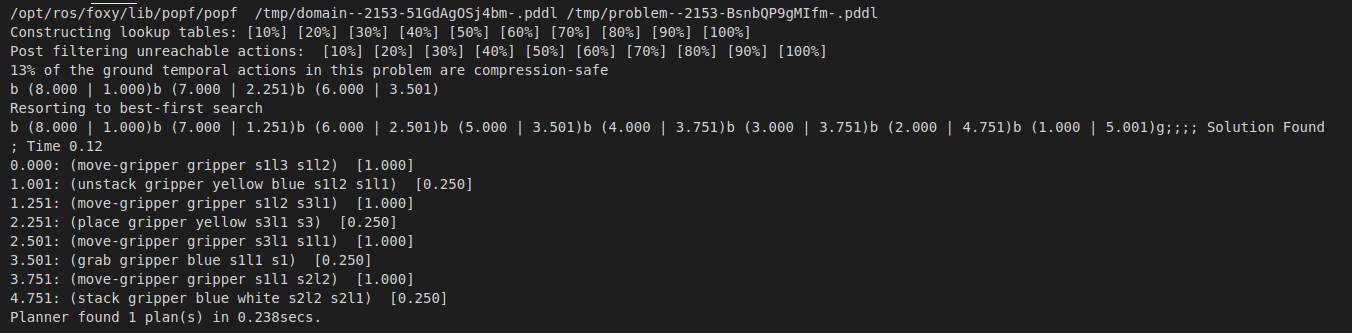
\includegraphics[width=\textwidth]{plugin_plan}
    \caption{Konsolenausgabe nach Ausführung des Planers über das \acs{PDDL}-Plugin}
    \label{fig:pluginplan}
\end{figure}

\begin{figure}[ht!]
    \centering
    \begin{minipage}[t]{0.45\linewidth}
        \centering
        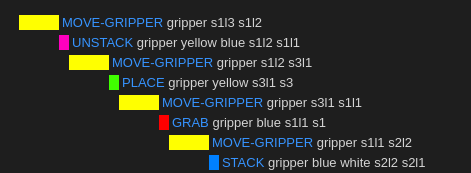
\includegraphics[width=\linewidth,keepaspectratio]{plugin_vis1}
    \end{minipage}% <- sonst wird hier ein Leerzeichen eingefügt
    \hfill
    \begin{minipage}[t]{0.45\linewidth}
        \centering
        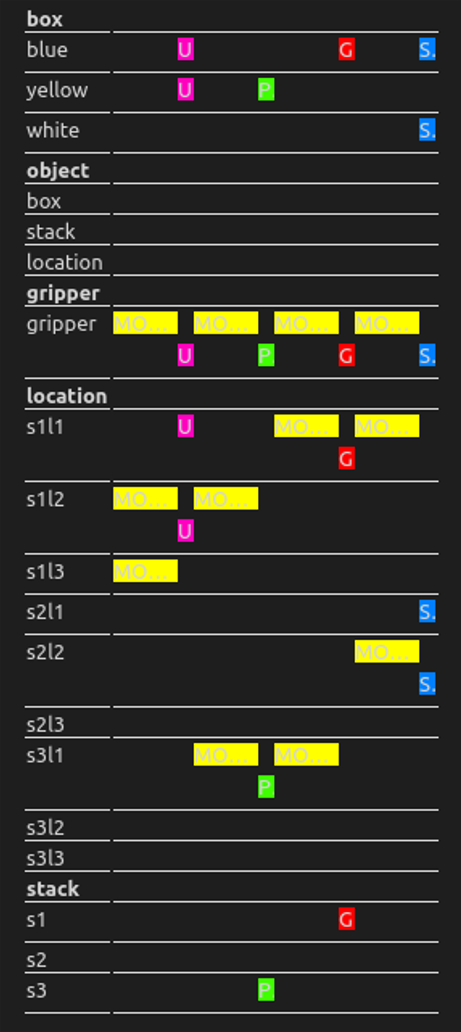
\includegraphics[width=.66\linewidth,keepaspectratio,valign=c]{plugin_vis3}
    \end{minipage}
    \title{Visualisierung eines Plans mit dem PDDL-Plugin}
    \caption{Visualisierung eines Plans mit dem \acs{PDDL}-Plugin mit Fokus auf die Aktionen (links) und relevante Objekte (rechts)}
    \label{fig:pluginvis}
\end{figure}
\subsubsection{Partial Order Planning}{\label{section:pop}}
\emph{\acf{POP}} ist eine Form des Planens, in dem die Aktionen eines Plans nur soweit geordnet sind, wie es notwendig ist \cite{dyer_2003}.
Dies steht im Gegensatz zu \emph{Total-Order} Planern wie \ac{STRIPS}.\\
Es wird nach dem emph{Principle Of Least Commitment} verfahren.
Das bedeutet, dass Entscheidungen soweit wie möglich aufgeschoben und erst getroffen werden, wenn es absolut nötig ist.
Dies umfasst nicht nur die Reihenfolge von Aktionen, sondern auch die Bindung von Variablen.\\
Ein Partial-Order Plan kann als 4-Tupel \cite{grastien} beschrieben werden.
\begin{itemize}
    \item eine Menge von Aktionen
    \item eine Menge von Einschränkungen der Reihenfolge
    \item eine Menge von kausalen Zusammenhängen
    \item eine Menge offener Vorbedingungen (Vorbedingungen einer Aktion, die nicht durch eine andere Aktion erfüllt werden)
\end{itemize}
Die Menge der Aktionen enthält Instanzen von Aktionen der Domäne.
Eine Aktion der Domäne kann daher mehrfach vorkommen.
Einschränkungen der Reihenfolge $A < B$ bilden ab, dass Aktion $A$ vor Aktion $B$ ausgeführt werden muss.
Zyklische Einschränkungen sind nicht erlaubt.
Ein kausaler Zusammenhang $A \xrightarrow{\alpha} B$ beschreibt, dass die Aktion $A$ die Vorbedingung $\alpha$ der Aktion $B$ erfüllt.\\
Die Suche erfolgt im Plan Space.
Jeder Knoten im Graph entspricht einem Teilplan und jede Kante einer Änderung des einen zum anderen Plan.
Dies kann durch das Hinzufügen eines weiteren Schrittes oder einer Einschränkung sowie der Bindung einer Variable geschehen.
Die Wurzel des Graphen besteht aus einem Plan mit zwei Schritten, die den Startzustand und das Ziel darstellen.
Der Startzustand wird durch eine Aktion repräsentiert, die keine Vorbedingungen und alle Fakten als Effekt hat.
Das Ziel erhält alle Zielfakten als Vorbedingung und hat keinen Effekt.
Zusätzlich enthält der Plan die Einschränkung, dass die Aktion für den Start vor der Aktion für das Ziel ausgeführt werden muss ($Start < Ziel$).\\
Ein Plan ist eine Lösung, wenn \cite{grastien}:
\begin{itemize}
    \item keine Aktion des Plans eine offene Vorbedingung hat
    \item und wenn keine Threats existieren
\end{itemize}
Ist der aktuelle Plan keine Lösung, werden folgende Schritte vorgenommen~\cite{grastien}:
\begin{itemize}
    \item eine offene Vorbedingung $p$ einer Aktion $B$ wählen
    \item eine existierende Aktion $A$, die die Vorbedingung $p$ erfüllt wählen oder eine neue Aktion $A$ erzeugen
    \item den kausalen Zusammenhang $A \xrightarrow{p} B$ und die Reihenfolge $A < B$ hinzufügen
    \item wenn $A$ eine neue Aktion ist, die Reihenfolge $Start < A$ hinzufügen
    \item Probleme zwischen dem neuen kausalen Zusammenhang und den existierenden Aktionen lösen sowie zwischen den existierenden kausalen Zusammenhang und $A$, wenn $A$ eine neue Aktion ist.
    \item entsteht durch das Hinzufügen der Reihenfolgen ein Zyklus, kann der Plan keine Lösung mehr werden
\end{itemize}
Ein Problem ist eine Beziehung zwischen einer Aktion $C$ und einem kausalen Zusammenhang  $A \xrightarrow{p} B$, bei der die Aktion $C$ einen Effekt $\neg p$ hat.
Sollte $C$ nach $A$ aber vor $B$ ausgeführt werden, ist die Vorbedingung $p$ für $B$ nicht mehr gegeben.
Probleme können durch \emph{Promotion} oder \emph{Demotion} gelöst werden~\cite{dyer_2003}.
Bei \emph{Promotion} wird der problematische Schritt $C$ nach dem kausalen Zusammenhang ausgeführt: die Reihenfolge $B < C$ wird hinzugefügt.
Bei \emph{Demotion} wird der problematische Schritt $C$ vor dem kausalen Zusammenhang ausgeführt: die Reihenfolge $C < A$ wird hinzugefügt.

\subsubsection{Forward Chaining Partial Order Planning}
Die Prinzipien des \ac{POP} sollen nun mit Vorwärtsverkettung kombiniert werden.
Für Vorwärtsverkettung mit einem Total-Order Plan können Zustände als Tupel $(F,V,Q,P,C)$ beschrieben werden~\citep{popf}:
\begin{itemize}
    \item F ist eine Menge von Fakten, die im Zustand gelten
    \item V enthält die Werte numerischer Variablen
    \item Q ist eine Liste von Aktionen, die begonnen haben, aber noch nicht beendet sind
    \item P ist der Plan, um den Zustand zu erreichen
    \item C ist eine Liste aller zeitlichen Einschränkungen der Schritte in $P$
\end{itemize}
Um eine Aktion zum Plan hinzuzufügen, müssen deren Start- und Endpunkte hinzugefügt werden.
Dies muss nicht in aufeinander folgenden Schritten geschehen.
Wird eine Aktion hinzugefügt werden $F$ und $V$ entsprechend der Effekte angepasst.
Die Voraussetzung, um eine Aktion hinzufügen zu können ist, dass $Q$ keine Aktion enthält, zu der die Effekte der neuen Aktion einen Konflikt darstellen würden.\\
Vorwärtsverkettung im Zustandsraum hat, durch den \emph{Total-Order} Plan, den Vorteil, dass nicht explizit nach Problemen gesucht werden muss.
Neue Aktionen werden immer am Ende hinzugefügt, wodurch sie kein Problem für die Vorbedingungen und Effekte früherer Aktionen darstellen können.
Gleichzeitig kann keine folgende Aktion ein Problem für diese darstellen.
Dieser Vorteil kommt mit dem Nachteil der frühen Bindung und einer festgelegten Reihenfolge zwischen Aktion, zwischen denen kein Zusammenhang besteht.\\
Es soll ein Kompromiss zwischen den Vorteilen von \emph{Total-} und \emph{Partial-Order} Planung gefunden werden.
Dem Tupel werden weitere Elemente hinzugefügt:
\begin{itemize}
    \item $F^+(F^-)$, wobei $F^+(p)(F^-(p))$ den Index eines Schrittes $a$ angeben, indem der Fakt $p$ als letztes hinzugefügt (oder gelöscht) wurde
    \item $FP$, wobei $FP(p)$ eine Menge von Paaren $\langle i,d \rangle \in (\mathbb{N}_0 \times \{0,\epsilon\})$:\\
    \begin{itemize}
        \item $\langle i,0 \rangle \in FP(p)$ beschreibt, dass Schritt $i$ am Ende eines offenen Intervalls liegt, in dem $p$ wahr sein muss.\\
        In \ac{PDDL} gibt es diese für Aktionen mit der \emph{over all} Bedingung $p$, wobei $i$ der Endpunkt dieser Aktion ist.
        \item $\langle i,\epsilon \rangle \in FP(p)$ beschreibt, dass Schritt $i$ der Start eines Intervalls ist, indem $p$ wahr sein muss.\\
        Dies entspricht \emph{at start} oder \emph{at end} Bedingungen in \ac{PDDL}, die relevant für den Schritt $i$ sind.
    \end{itemize}
\end{itemize}

\subsubsection{Partial Order Planning Forward}
\ac{POPF} ist ein am King’s College London entwickelter Planer, der die in Abschnitt~\ref{section:pop} genannten Methoden implementiert~\citep{popf}.
Als Heuristik wird ein temporaler \ac{RPG} genutzt.
Ein \acf{RPG} ist ein Planungsgraph, in dem versucht wird, ein vereinfachtes Problem zu lösen.
Die Vereinfachung besteht darin, alle negativen Effekte von Aktionen zu ignorieren.\\
Der Graph besteht aus einer Sequenz $F_0, A_0, ..., F_{t-1}, A_{t-1}, F_t, A_t$: Aktions- und Faktenschichten, die sich abwechseln.
Die Wurzel des Graphen ist eine Faktenschicht, die den aktuellen Zustand abbildet.
Eine Aktionsschicht enthält alle Aktionen, die in der vorhergehenden Faktenschicht anwendbar sind.
Eine Faktenschicht enthält alle Fakten, die durch alle Aktionen der vorhergehenden Aktionsschicht hinzugefügt werden.
Da nur positive Effekte betrachtet werden, enthält eine Faktenschicht auch alle Fakten der vorherigen Faktenschicht und eine Aktionsschicht ebenfalls alle Aktionen der vorherigen Aktionsschicht.\\
Ein Beispiel eines \ac{RPG} ist in Abbildung~\ref{fig:rpg} dargestellt.
Im Startzustand gelten die Fakten $at(Home)$ und $has(Money)$, dargestellt in $F_0$.
Die einzige Aktion, deren Vorbedingungen erfüllt ist, ist $move(Home, Shop)$ und wird der Aktionsschicht $A_0$ hinzugefügt.
Pfeile, die zu Aktionen gehen, zeigen die Fakten, die als Vorbedingung gelten.
Pfeile, die zu Fakten gehen, zeigen die Aktionen, durch deren Effekt sie hinzugefügt wurden.
In $F_1$ wird als Effekt der Aktion $move(Home, Shop)$ der Fakt $at(Shop)$ hinzugefügt.
Da negative Effekte ignoriert werden, gilt $at(Home)$ weiterhin.
Da in $F_1$ nun $at(Shop)$ und $has(Money)$ gelten, kann in $A_1$ die Aktion $buy(Product, Money)$ angewendet werden.
Dies resultiert in dem Fakt $has(Product)$ in $F_2$.\\
Angenommen, das Ziel ist $has(Product)$, so ist dieses Ziel in $F_2$ erfüllt.
Mit $t = 2$ als Wert der Heuristik, wird gezeigt, dass mindestens zwei Aktionen nötig sind um vom Startzustand zum Ziel zu gelangen.
Da $at(Home)$ vom Startzustand aus durchgängig gilt, erhält jedoch auch das Ziel $\{at(Home),has(Product)\}$ den Heuristikwert 2.\\
\begin{figure}[ht!]
    \centering
    \tikzset{every picture/.style={line width=0.75pt}} %set default line width to 0.75pt
    %\usetikzlibrary{arrows.meta}
    \begin{tikzpicture}[x=0.75pt,y=0.75pt,yscale=-1,xscale=1]
%uncomment if require: \path (0,355); %set diagram left start at 0, and has height of 355

%Shape: Rectangle [id:dp564712349225938]
        \draw  [fill={rgb, 255:red, 228; green, 250; blue, 206 }  ,fill opacity=1 ] (105,5) -- (550,5) -- (550,45) -- (105,45) -- cycle ;
%Rounded Rect [id:dp5993299884546457]
        \draw   (101,88) .. controls (101,83.58) and (104.58,80) .. (109,80) -- (540,80) .. controls (544.42,80) and (548,83.58) .. (548,88) -- (548,112) .. controls (548,116.42) and (544.42,120) .. (540,120) -- (109,120) .. controls (104.58,120) and (101,116.42) .. (101,112) -- cycle ;
%Shape: Rectangle [id:dp4448475604191735]
        \draw  [fill={rgb, 255:red, 228; green, 250; blue, 206 }  ,fill opacity=1 ] (105,150) -- (550,150) -- (550,190) -- (105,190) -- cycle ;
%Rounded Rect [id:dp06633752127787629]
        \draw   (102,228) .. controls (102,223.58) and (105.58,220) .. (110,220) -- (541,220) .. controls (545.42,220) and (549,223.58) .. (549,228) -- (549,252) .. controls (549,256.42) and (545.42,260) .. (541,260) -- (110,260) .. controls (105.58,260) and (102,256.42) .. (102,252) -- cycle ;
%Shape: Rectangle [id:dp8200443828072568]
        \draw  [fill={rgb, 255:red, 228; green, 250; blue, 206 }  ,fill opacity=1 ] (105,290) -- (550,290) -- (550,330) -- (105,330) -- cycle ;

% Text Node
        \draw (185,15) node [anchor=north west][inner sep=0.75pt]   [align=left] {at(Home)};
% Text Node
        \draw (395,15) node [anchor=north west][inner sep=0.75pt]   [align=left] {has(Money)};
% Text Node
        \draw (255,90) node [anchor=north west][inner sep=0.75pt]   [align=left] {move(Home,Shop)};
% Text Node
        \draw (175,160) node [anchor=north west][inner sep=0.75pt]   [align=left] {at(Home)};
% Text Node
        \draw (300,160) node [anchor=north west][inner sep=0.75pt]   [align=left] {at(Shop)};
% Text Node
        \draw (425,160) node [anchor=north west][inner sep=0.75pt]   [align=left] {has(Money)};
% Text Node
        \draw (105,230) node [anchor=north west][inner sep=0.75pt]   [align=left] {move(Home,Shop)};
% Text Node
        \draw (250,230) node [anchor=north west][inner sep=0.75pt]   [align=left] {move(Shop,Home)};
% Text Node
        \draw (394,230) node [anchor=north west][inner sep=0.75pt]   [align=left] {buy(Product,Money)};
% Text Node
        \draw (120,300) node [anchor=north west][inner sep=0.75pt]   [align=left] {at(Home)};
% Text Node
        \draw (235,300) node [anchor=north west][inner sep=0.75pt]   [align=left] {has(Money)};
% Text Node
        \draw (360,300) node [anchor=north west][inner sep=0.75pt]   [align=left] {at(Shop)};
% Text Node
        \draw (450,300) node [anchor=north west][inner sep=0.75pt]   [align=left] {has(Product)};
% Text Node
        \draw (30,20.4) node [anchor=north west][inner sep=0.75pt]    {$F_{0}$};
% Text Node
        \draw (30,93.4) node [anchor=north west][inner sep=0.75pt]    {$A_{0}$};
% Text Node
        \draw (30,160) node [anchor=north west][inner sep=0.75pt]    {$F_{1}$};
% Text Node
        \draw (30,230) node [anchor=north west][inner sep=0.75pt]    {$A_{1}$};
% Text Node
        \draw (30,300) node [anchor=north west][inner sep=0.75pt]    {$F_{2}$};
% Connection
        \draw[-{Latex[length=3mm]}]    (234.39,38) -- (301.47,84.85) ;
        %\draw [shift={(303.11,86)}, rotate = 214.94] [color={rgb, 255:red, 0; green, 0; blue, 0 }  ][line width=0.75]    (10.93,-3.29) .. controls (6.95,-1.4) and (3.31,-0.3) .. (0,0) .. controls (3.31,0.3) and (6.95,1.4) .. (10.93,3.29)   ;
% Connection
        \draw[-{Latex[length=3mm]}]    (330,111) -- (330,156) ;
        %\draw [shift={(352.31,157)}, rotate = 241.84] [color={rgb, 255:red, 0; green, 0; blue, 0 }  ][line width=0.75]    (10.93,-3.29) .. controls (6.95,-1.4) and (3.31,-0.3) .. (0,0) .. controls (3.31,0.3) and (6.95,1.4) .. (10.93,3.29)   ;
% Connection
        \draw[-{Latex[length=3mm]}]    (335,182) -- (331.25,227) ;
        %\draw [shift={(330.34,226)}, rotate = 296.9] [color={rgb, 255:red, 0; green, 0; blue, 0 }  ][line width=0.75]    (10.93,-3.29) .. controls (6.95,-1.4) and (3.31,-0.3) .. (0,0) .. controls (3.31,0.3) and (6.95,1.4) .. (10.93,3.29)   ;
% Connection
        \draw[-{Latex[length=3mm]}]    (340,182) -- (455,227) ;
        %\draw [shift={(450.05,228)}, rotate = 212.72] [color={rgb, 255:red, 0; green, 0; blue, 0 }  ][line width=0.75]    (10.93,-3.29) .. controls (6.95,-1.4) and (3.31,-0.3) .. (0,0) .. controls (3.31,0.3) and (6.95,1.4) .. (10.93,3.29)   ;
% Connection
        \draw[-{Latex[length=3mm]}]    (470.7,182) -- (470,227) ;
        %\draw [shift={(473.3,228)}, rotate = 286.93] [color={rgb, 255:red, 0; green, 0; blue, 0 }  ][line width=0.75]    (10.93,-3.29) .. controls (6.95,-1.4) and (3.31,-0.3) .. (0,0) .. controls (3.31,0.3) and (6.95,1.4) .. (10.93,3.29)   ;
% Connection
        \draw[-{Latex[length=3mm]}]    (474,253) -- (487,298) ;
        %\draw [shift={(487.21,299)}, rotate = 253.15] [color={rgb, 255:red, 0; green, 0; blue, 0 }  ][line width=0.75]    (10.93,-3.29) .. controls (6.95,-1.4) and (3.31,-0.3) .. (0,0) .. controls (3.31,0.3) and (6.95,1.4) .. (10.93,3.29)   ;

    \end{tikzpicture}
    \caption{\acl{RPG} für das Ziel $\{at(Home), has(Product)\}$}
    \label{fig:rpg}
\end{figure}
Die Erstellung des Graphen wird gestoppt, wenn eine Faktenschicht alle Ziele erfüllt oder wenn eine Faktenschicht der vorherigen entspricht.
Werden zwischen zwei Faktenschichten keine neuen Fakten hinzugefügt, können auch in zukünftigen Faktenschichten keine neuen Fakten mehr hinzugefügt werden.
Endet ein Graph auf diese Weise, ist das vereinfachte Problem nicht lösbar und der Zustand erhält einen Heuristikwert von \emph{unendlich}.
Andernfalls wird ein vereinfachter Plan aus dem Graphen extrahiert.
Die Länge des optimalen vereinfachten Plans ist eine zulässige Heuristik.
Der optimale Plan lässt sich jedoch nicht effizient extrahieren~\cite{hoffmannnebel2001}.
Daher wird ein suboptimaler Plan extrahiert, wodurch die Heuristik nicht mehr zulässig ist.\\
Um einen \ac{RPG} für temporales Planen zu erweitern, werden Aktionen in Startaktionen $A_\vdash$ und Endaktionen $A_\dashv$ aufgeteilt, die jeweils nur \emph{at start} und \emph{at end} Effekte enthalten.
Der Index $t$ einer Schicht entspricht nun einem Zeitstempel.\\
Als Suchverfahren wird zunächst \ac{EHC} versucht.
Der in Abbildung~\ref{fig:ehc_algo} beschriebene Algorithmus beginnt im Startzustand $S$.
\begin{figure}[h!]
           \centering
           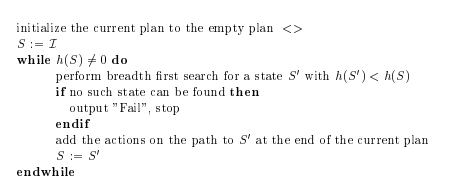
\includegraphics{ehc_algo}
           \caption{\acl{EHC} Algorithmus~\cite{hoffmannnebel2001}}
           \label{fig:ehc_algo}
\end{figure}
Von diesem aus wird wird eine \emph{breadth-first} Suche gestartet.
Diese findet den nächstbesten Nachfolger, also den nächsten Zustand $S'$, dessen Heuristik besser als die des aktuellen Zustands ist.
Gelingt dies, wird der Weg von $S$ nach $S'$ zum Plan hinzugefügt.
Die Suche wird gestoppt, wenn ein Zustand mit der Heuristik 0 gefunden wird.
Ist die Heuristik des aktuellen Zustands $\neq 0$ und wird kein Zustand mit einer besseren Heuristik gefunden, schlägt der Algorithmus fehl.
Zustände werden in einer \emph{Queue} gespeichert und für eine Iteration der Suche wird der erste Zustand $S'$ von dieser entfernt und und die Heuristik berechnet.
Die Suche ist erfolgreich, wenn die Heuristik für diesen Zustand $S'$ besser als die von $S$ ist.
Andernfalls werden die Nachfolger von $S'$ zum Ende der \emph{Queue} hinzugefügt.
Wiederholte Zustände werden durch ein \emph{HashTable} der bereits besuchten Zustände vermieden.
Die Suche schlägt fehl, wenn keine weiteren Zustände erreicht werden können.\\
Wird in einer Iteration kein besserer Zustand gefunden, stoppt \ac{EHC}, ohne eine Lösung zu finden.
Dies geschieht, da \ac{EHC} Entscheidungen, eine Aktion in den Plan aufzunehmen, nie rückgängig macht.
Der Algorithmus ist daher nur vollständig für Planungsaufgaben, die keine \emph{"dead ends"} enthalten.
Ein \emph{Dead End} für eine Planungsaufgabe $(O,I,G)$ ist definiert als ein Zustand $S$, der erreichbar ist und von diesem aus keine Plan das Ziel erreichen kann:\\
$\exists P: S = Result(I,P)$  und  $\neg\exists P': G\subseteq Result(S,P')$\\
Um die Vollständigkeit der Planung zu gewährleisten wird, im Fall eines Fehlschlags von \ac{EHC}, eine neue \emph{best-first} Suche ausgehend vom ursprünglichen Startzustand gestartet.
\subsubsection{Behavior Tree}
\acp{BT} sind ein modulares System, das in der Videospieleindustrie entwickelt wurde~\cite{bt_book}.
Sie ermöglichen aus simplen Aktionen komplexe Verhaltensmuster zu modellieren ohne das Aktionen Kenntnis über andere Aktionen haben müssen~\cite{bt_robotics}.
Entsprechend~\cite{bt_1} ist ein \ac{BT} ein gerichteter azyklischer Graph $G(V,E)$ mit $|V|$ Knoten und $|E|$ Kanten.
Ein Elternknoten von einem Paar verbundener Knoten ist der, von dem die Kante ausgeht.
Der Knoten mit der eingehenden Kante ist ein Kindknoten.
Knoten ohne Kinder heißen Blätter.
Ein Knoten ohne Eltern heißt Wurzel.
In einem \ac{BT} gibt es genau eine Wurzel mit genau einem Kind.\\
Nach~\cite{bt_book} beginnt die Ausführung eines \ac{BT} bei der Wurzel, die in einem bestimmten Intervall ein Signal erzeugt, dass die Ausführung eines Knoten erlaubt (''tick'').
Dieses Signal wird an das Kind der Wurzel gesendet.
Ein Knoten wird ausgeführt, wenn es dieses Signal erhält und auch nur dann.
Wird ein Knoten ausgeführt, gibt er einen Status zurück.
Der Status ist einer von drei möglichen~\cite{bt_uav}:
\begin{itemize}
    \item Running: die Ausführung läuft noch
    \item Success: die Ausführung war erfolgreich
    \item Failure: die Ausführung ist fehlgeschlagen
\end{itemize}\\
Wie in~\cite{bt_1} beschrieben, werden verschiedene Arten von Knoten auf verschiedene Typen beschränkt.
Blätter sind Ausführungsknoten und haben einen der folgenden Typen:
\begin{itemize}
    \item Aktion
    \item Bedingung
\end{itemize}
Knoten mit Kindern, mit Ausnahme der Wurzel, sind Kontrollflussknoten und haben einen der folgenden Typen:
\begin{itemize}
    \item Selektor
    \item Sequenz
    \item Parallel
    \item Dekorator
\end{itemize}
Ein Selektor-Knoten führt seine Kinder der Reihe nach aus, bis das erste einen Status \emph{Running} oder \emph{Success} zurückgibt.
Nachfolgende Kinder werden dann nicht mehr ausgeführt und der Selektor gibt den entsprechenden Status zurück.
Wurden alle Kinder ausgeführt und keins hat einen Status \emph{Running} oder \emph{Success} zurückgegeben, gibt der Selektor den Status \emph{Failure} zurück.\\
Ein Sequenz-Knoten führt seine Kinder der Reihe nach aus, bis das erste einen Status \emph{Running} oder \emph{Failure} zurückgibt.
Nachfolgende Kinder werden dann nicht mehr ausgeführt und die Sequenz gibt den entsprechenden Status zurück.
Wurden alle Kinder ausgeführt und keins hat einen Status \emph{Running} oder \emph{Failure} zurückgegeben, gibt die Sequenz den Status \emph{Success} zurück.\\
Ein Parallel-Knoten führt alle Kinder aus, ohne auf den Status des vorherigen zu warten.
Überschreitet die Anzahl der Kinder, die \emph{Success} zurückgeben einen benutzerdefinierten Wert $S$, gibt der Knoten \emph{Success} zurück.
Haben $N-M+1$ Kinder \emph{Failure} zurückgegeben, wobei $N$ die Anzahl der Kinder ist, wird \emph{Failure} zurückgeben, da der Wert $S$ nicht mehr erreicht werden kann~\cite{bt_book}.
Alternativ kann ein zweiter benutzerdefinierter Wert $F$ eingeführt werden.
Überschreitet die Anzahl der Kinder, die \emph{Failure} zurückgeben diesen Wert $F$, wird direkt \emph{Failure} zurückgegeben~\cite{bt_1}.
$S$ und $F$ müssen $\leq M$ sein.
Wird keiner dieser beiden Werte überschritten, wird \emph{Running} zurückgegeben.\\
Ein Dekorator-Knoten hat genau ein Kind.
Er kann durch eine Bedingung entscheiden, ob das Kind ausgeführt wird und kann einen modifizierten Status zurückgeben.
Beispiele für Dekoratoren sind~\cite{bt_book}:
\begin{itemize}
    \item Invertierung/Negation: der \emph{Success} und \emph{Failure} Status des Kinds wird invertiert
    \item Zeitbeschränkung: gibt das Kind den Status \emph{Running} für länger als eine benutzerdefinierter Zeitspanne $T$ zurück, wird \emph{Failure} zurückgegeben und das Kind nicht mehr ausgeführt
\end{itemize}

\begin{table}[]
    \resizebox{\textwidth}{!}{%
        \begin{tabular}{|l|l|lll|}
            \hline
            \multicolumn{1}{|c|}{\multirow{2}{*}{\textbf{Knoten}}} &
            \multirow{2}{*}{\textbf{Symbol}} &
            \multicolumn{3}{c|}{\textbf{Rückgabewert}} \\ \cline{3-5}
            \multicolumn{1}{|c|}{} &
            &
            \multicolumn{1}{l|}{\textbf{Success}} &
            \multicolumn{1}{l|}{\textbf{Failure}} &
            \textbf{Running} \\ \hline
            Selektor &
            \multicolumn{1}{|c|}{?} &
            \multicolumn{1}{l|}{\begin{tabular}[c]{@{}l@{}}Wenn 1 Kind ''Success'' \\ zurückgibt\end{tabular}} &
            \multicolumn{1}{l|}{\begin{tabular}[c]{@{}l@{}}Wenn alle Kinder ''Failure''\\ zurückgeben\end{tabular}} &
            \begin{tabular}[c]{@{}l@{}}Wenn 1 Kind ''Running''\\ zurückgibt\end{tabular} \\ \hline
            Sequenz &
            \multicolumn{1}{|c|}{$\rightarrow$} &
            \multicolumn{1}{l|}{\begin{tabular}[c]{@{}l@{}}Wenn alle Kinder ''Success''\\  zurückgeben\end{tabular}} &
            \multicolumn{1}{l|}{\begin{tabular}[c]{@{}l@{}}Wenn 1 Kind ''Failure''\\ zurückgibt\end{tabular}} &
            \begin{tabular}[c]{@{}l@{}}Wenn 1 Kind ''Running''\\ zurückgibt\end{tabular} \\ \hline
            Parallel &
            \multicolumn{1}{|c|}{$\rightrightarrows$} &
            \multicolumn{1}{l|}{\begin{tabular}[c]{@{}l@{}}Wenn $\geq M$ Kinder ''Success''\\  zurückgeben\end{tabular}} &
            \multicolumn{1}{l|}{\begin{tabular}[c]{@{}l@{}}Wenn $> N - M$ Kinder ''Failure''\\ zurückgeben\end{tabular}} &
            \begin{tabular}[c]{@{}l@{}}Wenn keine der Bedingungen\\  für ''Success'' oder ''Failure'' \\ erfüllt sind\end{tabular} \\ \hline
            Dekorator &
            \multicolumn{1}{|c|}{$\lozenge$} &
            \multicolumn{1}{l|}{benutzerdefiniert} &
            \multicolumn{1}{l|}{benutzerdefiniert} &
            benutzerdefiniert \\ \hline
            Bedingung &
            \multicolumn{1}{|c|}{
                \begin{tikzpicture}
                    \draw[black!100] (0,0) -- (1,0);
                    \node[ellipse,draw] at (-0,-0.5) {Text};
                \end{tikzpicture}} &
            \multicolumn{1}{l|}{Wenn wahr} &
            \multicolumn{1}{l|}{Wenn falsch} &
            Nie \\ \hline
            Aktion &
            \multicolumn{1}{|c|}{
                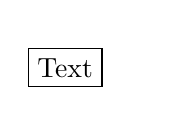
\begin{tikzpicture}
                    \draw[white] (0,0) -- (1,0);
                    \node[draw] at (0,-0.5) {Text};
                \end{tikzpicture}} &
            \multicolumn{1}{l|}{Bei vollständiger Ausführung} &
            \multicolumn{1}{l|}{\begin{tabular}[c]{@{}l@{}}Wenn vollständige Ausführung\\ nicht möglich ist\end{tabular}} &
            Während der Ausführung \\ \hline
        \end{tabular}%
    }
    \caption{Übersicht der \acs{BT} Knoten, nach~\cite{bt_book}}
    \label{tab:btoverview}
\end{table}

- Visualisierungs bsp.\\
\subsection{Planung in \ac{ROS2}}
Für die Planung in \ac{ROS2} wird \ac{PlanSys2} genutzt.
In diesem Abschnitt wird das in~\cite{plansys} beschriebene System zusammenfassend beschrieben.
Es wird dabei jedoch nur auf die für diese Arbeit relevanten Teile eingegangen.\\
\ac{PlanSys2} ist ein modulares OpenSource Planungsframework.
Ursprünglich als Nachfolger für ROSPlan~\cite{rosplan} geplant, bietet es viel umfangreichere Funktionen.
Hierfür werden unter anderem neue Funktionen von \ac{ROS2} wie LifeCycle-Knoten oder Multicast Kommunikation genutzt.\\
Eins der Designprinzipien bei der Entwicklung von \ac{PlanSys2} ist Modularität und Erweiterbarkeit.
Alle Komponenten haben klar definierte Schnittstellen, wodurch sie einfach erweitert oder ausgetauscht werden können.\\
Die Hauptkomponente ist der \emph{''Planner''} Knoten, der den tatsächlichen Planer aufruft.
Verschiedene Planer können über Plugins aufgerufen werden, die beschreiben, wie der Planer aufzurufen ist und wie der generierte Plan zu verstehen ist.
Standardmäßig sind \ac{POPF} sowie TFD (\emph{Temporal Fast Downward})~\cite{tfd} verfügbar und konfiguriert.\\
Der \emph{''Domain Expert''} Knoten liest die Domäne im \ac{PDDL}-Format ein.
Er kann mehrere verschiedene Domänen zu einer kombinieren.
Dies ermöglicht es, mehrere modulare Packages zu nutzen, die jeweils nur den für sie relevanten Teil einer Domäne beinhalten sowie deren Aktionen  implementieren.
Der Knoten dient zur Validierung (z.B. ob ein Prädikat, das hinzugefügt werden soll, mit den gegeben Objekten gültig ist) und dem Planer die Domäne zur Verfügung zu stellen.\\
Der \emph{''Problem Expert''} Knoten enthält alle Informationen zum gegebenen Problem: Objekte, Prädikate, Funktionen und Ziele.
Diese werden immer über den \emph{''Domain Expert''} validiert.
Wenn ein Plan angefordert wird, werden die gespeicherten Informationen zu einem Problem im \ac{PDDL} Format konvertiert und dem \emph{''Planner''} Knoten zur Verfügung gestellt.\\
Der \emph{''Executor''} Knoten ist dafür zuständig einen generierten Plan auszuführen.
Der Plan wird in einen \ac{BT} konvertiert, der diesen ausführt.\\
Ein weiteres Konzept ist die Unterstützung für mehrere Roboter sowie eine Spezialisierung bei der Ausführung von Aktionen.
Alle Knoten im gleichen Netzwerk können miteinander kommunizieren.
Es kann mehrere Knoten geben, die die gleiche Domänenaktion ausführen, sich aber auf bestimmte Parameter spezialisieren.
Mehrere Roboter können einen Knoten für die gleiche Aktion \emph{(move roboter start ziel)} ausführen, wobei sich jede darauf spezialisiert, die Aktion auszuführen, deren erster Parameter mit dem entsprechenden Roboter übereinstimmt.
Die gleiche Aktion kann je nach vorhandenen Parametern von verschiedenen Knoten ausgeführt werden.\\
\acp{BT} eignen sich für die Ausführung eines Plans, da sich mit ihnen sehr gut sequentielle und parallele Vorgänge beschreiben lassen.
Zunächst wird von einem Plan ein Ausführungs-Graph erstellt, der die Abhängigkeiten zwischen Aktionen zeigt.
Von diesen lässt sich ableiten, welche Aktionen parallel ausgeführt werden können und welche sequentiell ausgeführt werden müssen.
Semantisch entspricht jedes Blatt im Graphen einer Aktion.
In der Praxis ist jedes Blatt ein eigenständiger \ac{BT}, der nicht nur die selbst Aktion ausführt, sondern auch die Bedingungen überprüft und die Effekte ausführt (s. Abbildung~\ref{fig:plansysbtaction}).\\
\begin{figure}
    \centering
    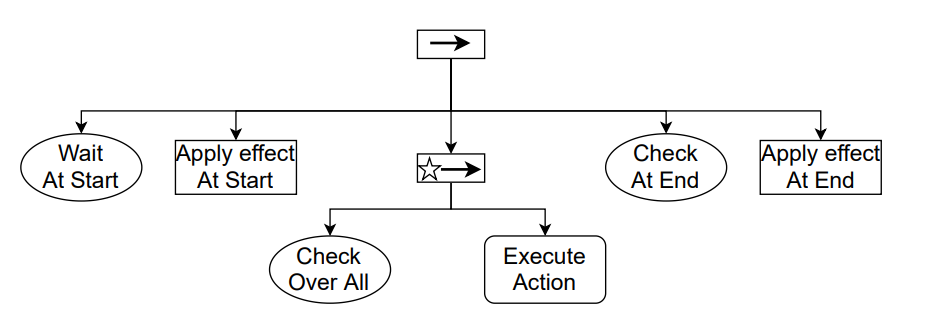
\includegraphics[width=\textwidth]{plansys2btaction}
    \caption{\acs{BT} zur Ausführung einer spezifischen Aktion~\cite{plansys}}
    \label{fig:plansysbtaction}
    \end{figure}
\ac{PlanSys2} hat drei große Limitationen.
\ac{PDDL}-Unterstützung beschränkt sich aktuell auf \ac{PDDL} 2.1 mit dem Ziel zukünftig, die aktuellste Version zu unterstützen.
Wird eine Aktion und damit ein Plan abgebrochen, gibt es keine Garantie, dass der Zustand der Welt konsistent bleibt.
Die Fähigkeit von Planern, die zunächst einen allgemeinen Plan liefern und diesen während der Ausführung verbessern, wird nicht genutzt.
Eine geplante Funktion ist jedoch, Übergänge von der Ausführunge eines Plans zu einem anderen zu ermöglichen.